\subsection*{\textbf{RQ2: Is there relationship between log change and resolution time of bug fixes?}}


\subsubsection*{\textbf{Motivation}}

In RQ1, we find that logs are changed more frequently in bug fixes. However, we do not know if leveraging and changing logs is beneficial during bug fixes. To answer this, we look at the  effort spent to fix the bug. We measure effort spent based on the time taken to resolve a bug, the number of developers involved during the resolution of a bug and the number of discussions posts on JIRA. We try to find whether there is a relationship between resolution time, developer involvement and log churn during bug fixes. 


\subsubsection*{\textbf{Approach}}

To find out whether there is a relationship between log churn and resolution time of bug fixes, we collect all JIRA issues with type `bug' from the three studied systems. We obtained the code commits for each of these JIRA issues by searching for the issue id from the commit messages. We identify the log churn, and the code churn for fixing each issue. We then split the JIRA issues into (1) bugs that are fixed with log churn and (2) bugs that are fixed without log churn. We use the code churn to measure the complexity of the issue. We then extracted three metrics from JIRA issues to measure the effort of fixing a bug:

\begin{enumerate}
	\item \textbf{Resolution time:} This metric measures how fast the bug is fixed. This metric is defined as the time taken from when the bug is opened until it is resolved. For example, if a bug was opened on 1$ ^{st}$ February 2015 and closed on 5$ ^{th}$ February 2015, the resolution time of the bug is four days. 
	
	\item \textbf {\# of comments:} This metric measures how much discussion is needed to fix a bug. Intuitively, the more discussion in an issue report, the more effort is spent on fixing the bug. We count the total number of comments in the discussion of each issue report.
	
	\item \textbf {\# of developers:} This metric measures the number of developers who participate in the discussion of fixing the bug. Intuitively, more developers who discuss the bug, more effort is spent on fixing the bug. We count the number of unique developers who comment on the issue report. We use the user names in the JIRA discussion to identify the developers. 
\end{enumerate}

Prior research has shown that complexity of software can be measured using different metrics, including source lines of code change~\cite{complexity}. Intuitively, a complex bug fix might have more code churn and in turn takes longer time to be resolved, more developers being involved and more discussions on JIRA. Therefore, we use code churn to normalize the resolution time, the number of comments, and the number of developers  during bug fixes. We use these normalized effort metrics to find if there is statistically significant difference between bug fixes with log churn and bug fixes without log churn. We use the {\em MannWhitney U} test to find the $|\rho|$ values and \textsl{Cohen's d} test to measure the effect size, similar to RQ1. 


\begin{table*}
	\caption{Comparing code and developer metrics between the bug fixes with log churn and bug fixes without log churn. The p-value is from MannWhitney U tests and the effect sizes are calculated using Cohen's d. P-values are smaller than 0.05 and negative effect size implies that metrics for bug fixes without log churn have higher values.}
	\label{tab:bugfixes}
	\centering{}%
	\begin{tabular}{|>{\centering}p{.12\textwidth}|c|>{\centering}p{.1\textwidth}|c|>{\centering}p{.1\textwidth}|c|>{\centering}p{.1\textwidth}|}
		\hline 
		\multirow{2}{*}{Metrics}& \multicolumn{2}{c|}{Hadoop} & \multicolumn{2}{c|}{HBase} & \multicolumn{2}{c|}{Qpid}\tabularnewline
		\cline{2-7} 
		
		& p-values  & Effect size & p-values  & Effect Size & p-values  & Effect size\tabularnewline
		\hline 
		Code churn & \textbf{ $<$2.2e-16} & 0.178 (small) & \textbf{$<$2.2e-16} & 0.023 &  \textbf{$<$2.2e-16} & 0.155\tabularnewline
		\hline 
		Resolution time & \textbf{4.7e-14} &  -0.095 & \textbf{$<$2.2e-16} & -0.188 (small) & \textbf{ 7.7e-08} & -0.276 (small)\tabularnewline
		\hline 
		\# of comments & \textbf{2.2e-16} & -0.573 (small) &  \textbf{$<$2.2e-16} &-0.436 (small) & \textbf{$<$2.2e-16} & -0.304 (small)\tabularnewline
		\hline 
		\# of developers & \textbf{ $<$2.2e-16} & -0.539 (small) & \textbf{$<$2.2e-16}& -0.617 (medium) & \textbf{$<$2.2e-16} & -0.440 (small)\tabularnewline
		\hline 
	\end{tabular}
\end{table*}
 
 \begin{figure*}[t]
 	\centering
 	\caption{Boxplot of code churn of bug fixes with log churn (shown in blue) against bug fixes without log churn (shown in grey).}
 	\label{fig:figure3}
 	
 	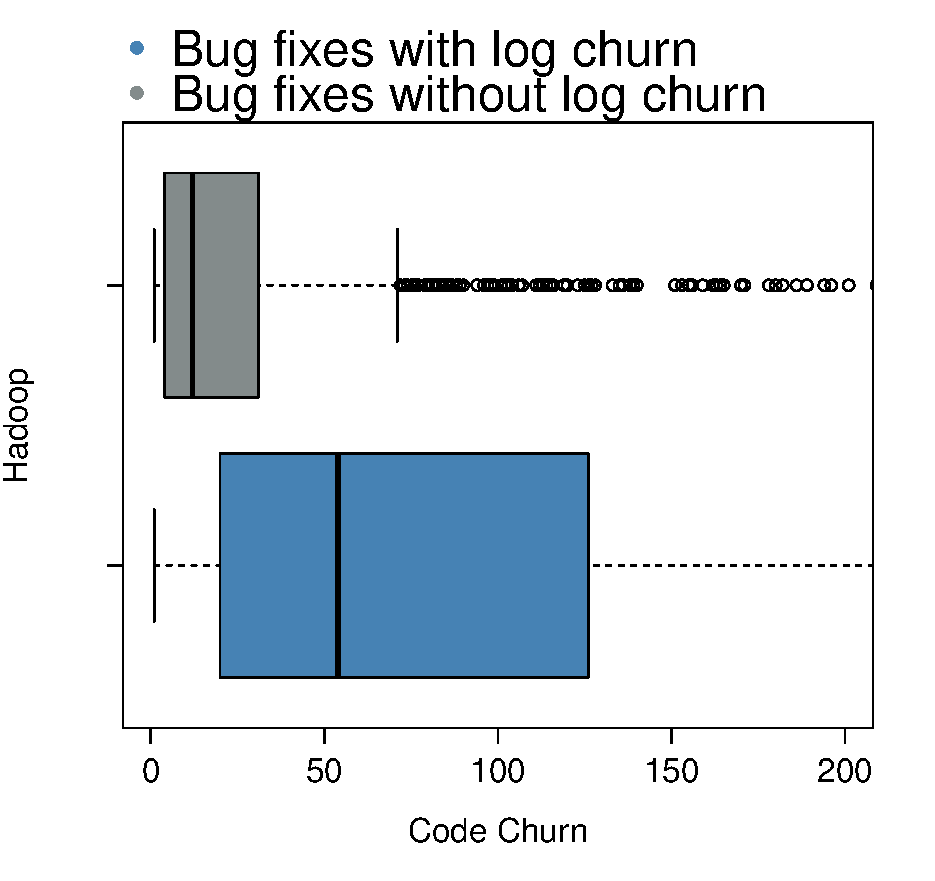
\includegraphics[width=.49\textwidth]{HadoopBoxPlot}
 	\hfill
 	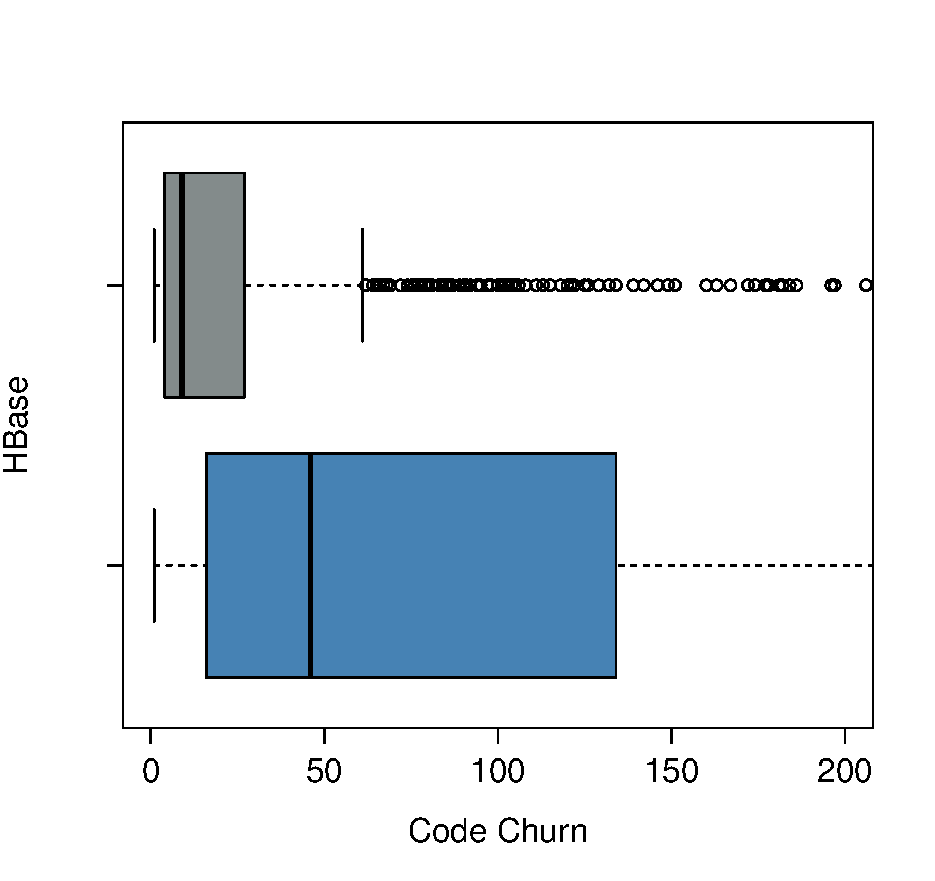
\includegraphics[width=.49\textwidth]{HBaseBoxPlot}\hfill
 	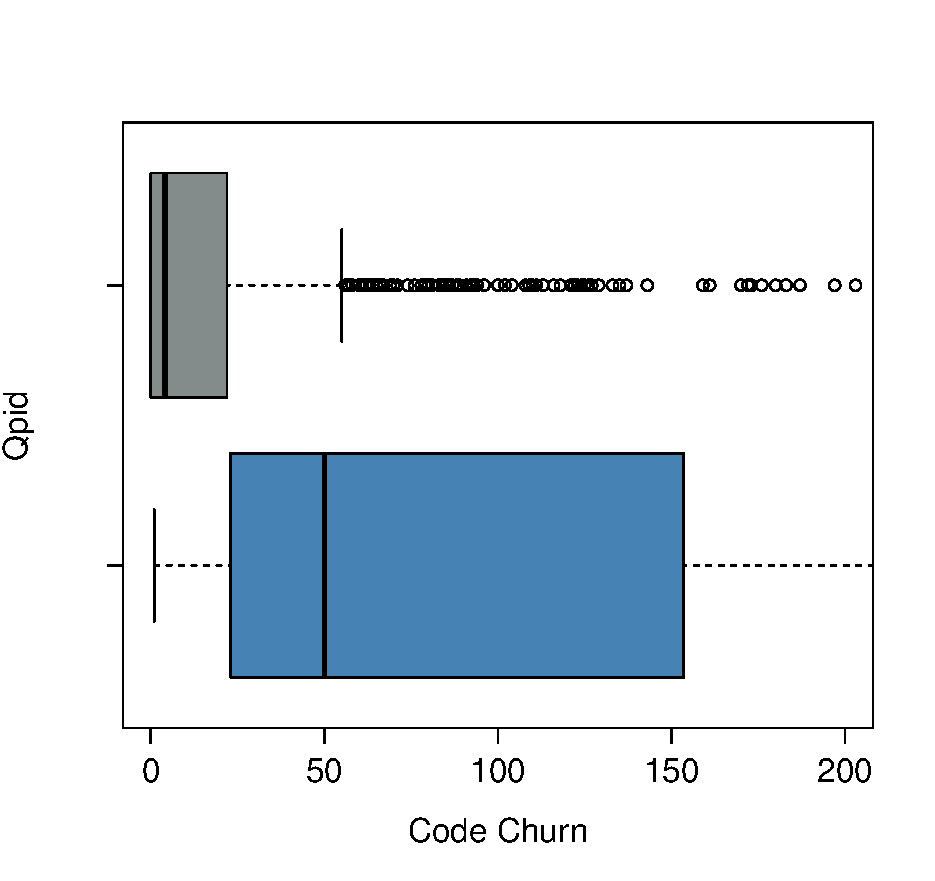
\includegraphics[width=.49\textwidth]{QpidBoxPlot}
 	
 \end{figure*}


\subsubsection*{\textbf{Results}}

\textbf{We find that the logs changes are more likely to occur during complex bugs fixes}. We find that the average code churn for fixing bugs is significantly higher with log churn than without log churn (see Table~\ref{tab:bugfixes} and Figure~\ref{fig:figure3}). This suggests that complex bug fixes are more likely to have log churn (statically significant with non-trivial effect size). 




\textbf{We find that bugs that are fixed with log churn, take shorter time with fewer comments and fewer people.} After normalizing the code churn, we find that the resolution time, the number of comments and the number of developers are all statistically significantly smaller in the bug fixes with log churn than the ones without log churn. This result suggests that given two bugs of the same complexity, the one with log churn usually take less time to get resolved and needs a fewer number of developers involved with fewer discussions. Changing logs may provide useful information to assist developers in discussing, diagnosing and fixing bugs. For example, when fixing bug HBASE-3074\footnote{https://issues.apache.org/jira/browse/HBASE-30741}, developers left the first comment to provide additional details in the log about where the failure occurs. In the source code, developers add the name of the servers into the the logs. Such additional data helps diagnose the cause of the failure and helps fix the bug.

To further understand how developers change logs during bug fixes, we conduct a manual analysis. We collected all the bug fixes with log changes for our studied systems. We selected a 5\% random sample (266 for \textsl{HBase}, 268 for \textsl{Hadoop} and 83 for \textsl{Qpid}) from all the commits. For the sampled commits, we manually examine the code changes and the corresponding JIRA issue reports to find the reasons of changing logs during bug fixes. We follow an iterative process, similar to prior research~\cite{seaman1999qualitative}, until we cannot find any new reasons. We find three reasons of changing logs during bug fixes as shown in Table~\ref{tba:LogUsage}. These three reasons may co-occur within a single commit. 

% The code changes are analyzed to identify common patters of log usage during debugging and JIRA issue reports are analyzed to understand the extent of log usage by developers.
\begin{table}[tbh]
	\protect\caption{Log change reasons during bug fix}
	\label{tba:LogUsage}	
	\begin{centering}
		\begin{tabular}{|>{\centering}p{2.5cm}|>{\centering}p{1.3cm}|>{\centering}p{1.3cm}|>{\centering}p{1.3cm}|}
			\hline 
			Projects & Hadoop & HBase & Qpid\tabularnewline
			\hline 
			\hline 
			Bug diagnosis & 157 & 175 & 49\tabularnewline
			\hline 
			Similar bugs detection & 156 & 170 & 42\tabularnewline
			\hline 
			Code quality assurance for bug fixes & 93 & 78 & 18\tabularnewline
			\hline 
		\end{tabular}
		\par\end{centering}
	
\end{table}
\begin{itemize}
	

\item \textbf{Bug diagnosis.} Developers change logs to print extra or different information into logs during the execution of the system. Such information is printed to ease bug diagnosis.
%The log changes in the category have added and deleted code prior to log changes (i.e., code block is changed). 
For example, HADOOP-2725\footnote{https://issues.apache.org/jira/browse/HADOOP-2725} is reported when users find that after copying a 100TB file across two clusters, the file sizes has a discrepancy of 6GB. However, the existing logs do not have proper format to show the size of the copied data. To help diagnose the bug, developers modify the logged variable to print the sizes of the copied data into a better format. %These log changes are committed along with bug fix, as it clarifies the log output and helps in understanding the logging context.

 %These findings are consistent with prior findings where majority of log changes are made during debugging~\cite{EMSEIAN}.

\item \textbf{Similar bugs detection.} After fixing a bug, developers may insert log into the code in order to monitor the execution of the system to detect similar bugs in the future. During the bug fixes, developers identify root-causes of the bug. After fixing the bug, developers change logs to capture the run-time event that may correspond to the root-cause of the bug, in order to identify future occurrence of a similar bug. The changed information in logs is not leveraged to fix the bug, but rather monitoring the systems for detecting a similar bug in the future. We find that logs in this category are mainly new logs being added into the system, unlike bug diagnosis which is mainly log modifications. 
%Log changes in this category have addition of new blocks (i.e., if, if-else, try-catch and exception) with higher code addition than deletion. 
For example, to fix HADOOP-2890\footnote{https://issues.apache.org/jira/browse/HADOOP-2890}, developers identify the reason behind blocks getting corrupted as an run-time exception. In the commit, we observe that the developers fix this bug and add \textsl{try catch} block with new logs to catch these exceptions. Such log will notify developers if a similar bug appears.

\item \textbf{Code quality assurance for bug fixes.} Sometime, developers need to introduce a large amounts of code to fix a bug. The introduction of bug-fixing code, may also introduce new bugs into the system. To ensure the quality of these bug fixes, developers insert new logs into the bug-fixing code. For example, in HBASE-3787\footnote{https://issues.apache.org/jira/browse/HBASE-3787}, developers encounter a non-idempotent operation (i.e., running the operation more than once produces different results) that causes an error in the application. The fix of this bug involves over 13 developers and 112 discussions over the two years. The developers add several new files and functions during the bug fix, and added logs to assure the code quality of the fix. 
\end{itemize}



\hypobox{Logging statements are changed during fixing more complex bugs. After normalizing the complexity of bugs using code churn, we find that bug fixes with log churn are resolved faster with fewer people and fewer discussions.}

